\chapter{Background estimation}\label{chap:Backgr}
\minitoc


\begin{table}[!b]
    \caption{Background processes with their associated cross sections and uncertainties (if given). The quoted cross sections are used to normalise estimates of expected number of events}
	\label{tab:Backgrounds}
	\begin{center}
		\begin{tabular}{c | c | c}
		\hline
		\hline
		Process & $\sigma \cdot BR (\pm unc.)$ [pb] & Order \\
\hline
$W^+ \to l \nu$ & \WPxsec ($\pm \WPxsecUncertanty$) & NNLO \\ 
$W^- \to l \nu$ & \WMxsec ($\pm \WMxsecUncertanty$) & NNLO \\ 
\hline
$Z \to ll$ & \Zxsec($\pm \ZxsecUncertanty$) & NNLO \\
$Z \to \tau\tau$  & \Zxsec & LO \\
\hline
$t \bar{t}$ & \Ttxsec & LO \\
$WW$ & \WWxsec & LO \\
$ZZ$ & \ZZxsec & LO \\
$WZ$ & \WZxsec & LO \\
\hline
\hline
\end{tabular}
\end{center}    
\end{table}


After the event selection described in Chap. \ref{chap:EventSelection} the background contribution is around 4\% for W-analysis and 0.2\% for Z analysis (which with this statistics is  negligible). Main backgrounds for W analysis are coming from:
\begin{itemize}
\item Processes with $\tau$ lepton, misidentified as an electron or muon + missing energy from neutrino
\item Z decays with one missing lepton.
\item QCD processes. In electron channel these are mostly jets faking electrons, while in the muon channel it consists mainly of a real muons produced in decays of heavy-flavor mesons. %The $E_T^{miss}$ distribution is peaking
\end{itemize}
Most of the backgrounds are estimated using MC. They are normalized using highest cross-section order available. The total list of simulated backgrounds and its cross-section is shown in a Table \ref{tab:Backgrounds}. The QCD background is estimated using data driven method.


\section{QCD background estimation}\label{sec:QCD}


\begin{figure}[!tbp]
\begin{minipage}[h]{0.49\linewidth}
\center{ 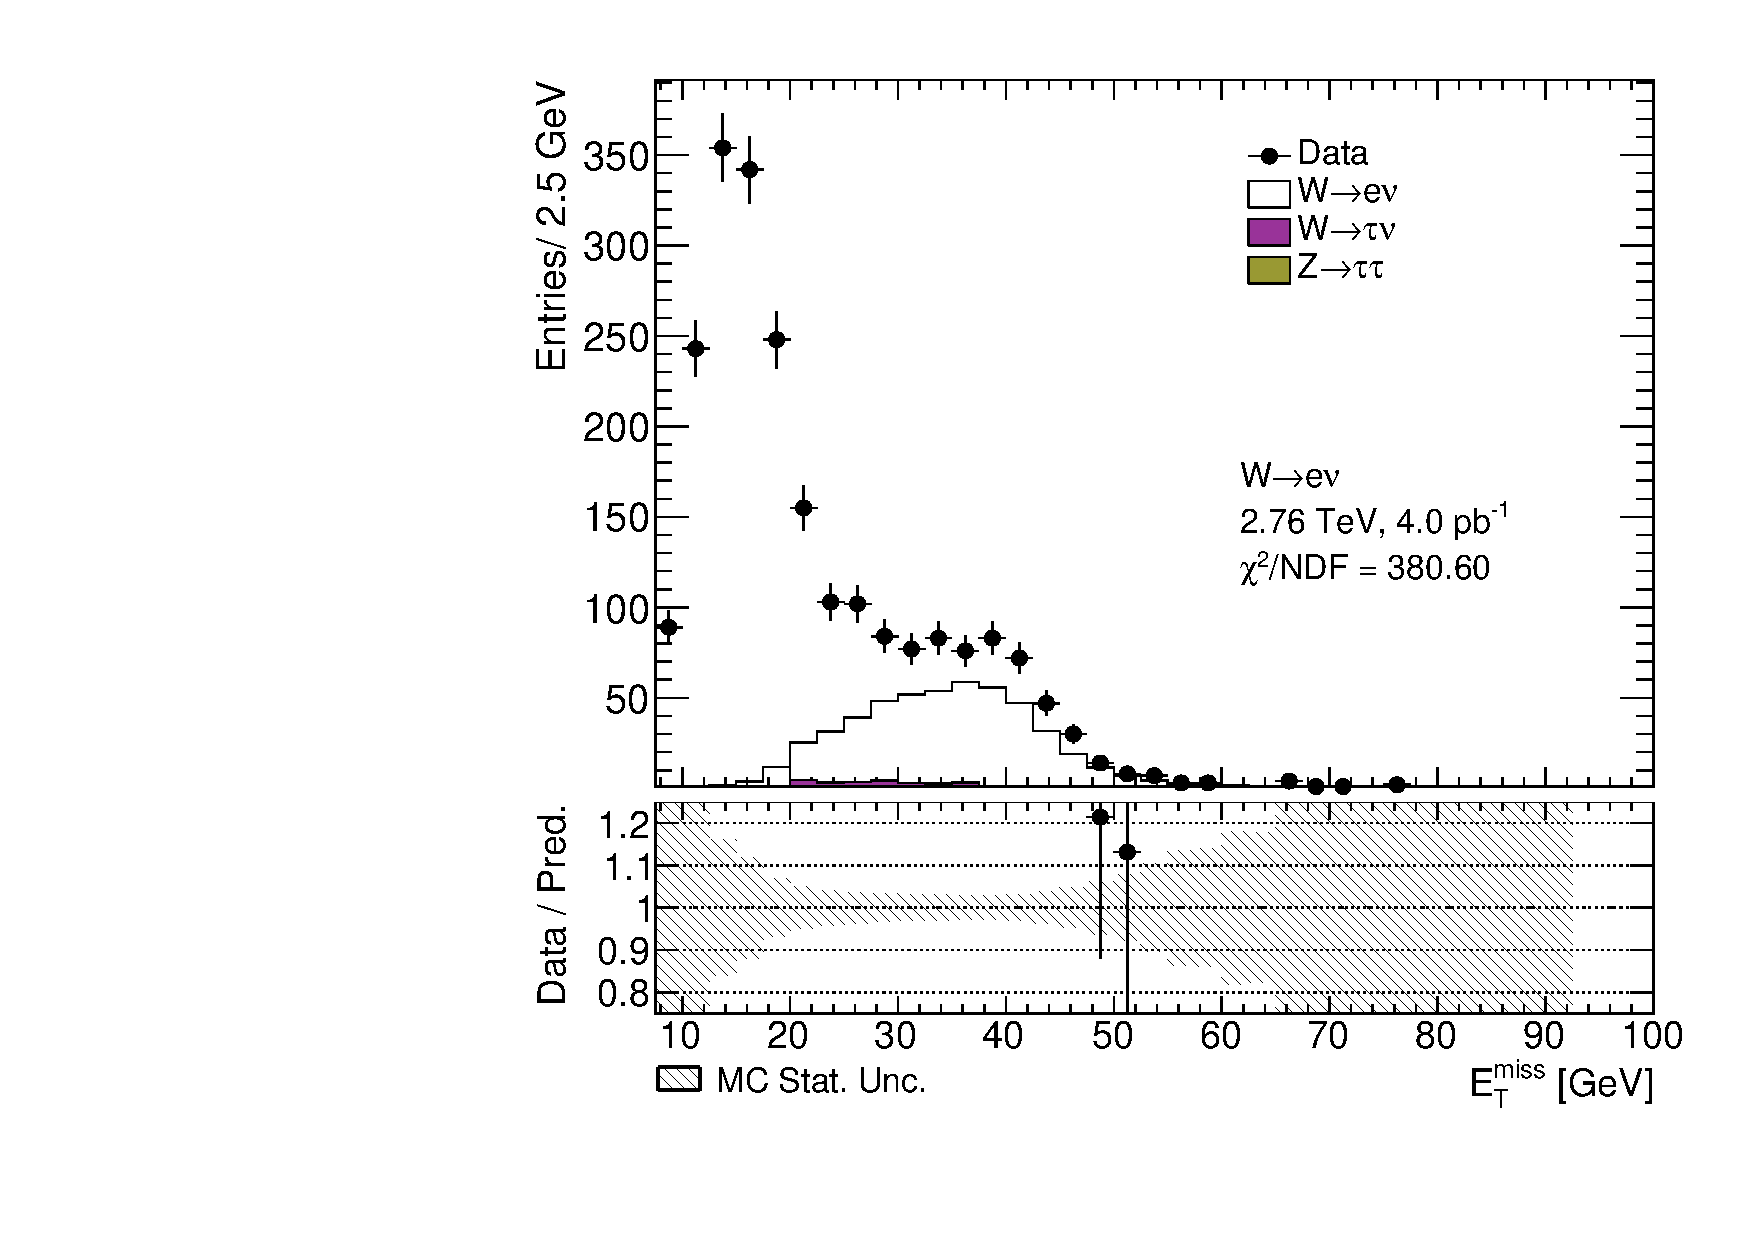
\includegraphics[width=1.\linewidth]{QCD/QCDetMissTempl.pdf} \\a)}
\end{minipage}
\hfill
\begin{minipage}[h]{0.49\linewidth}
\center{ 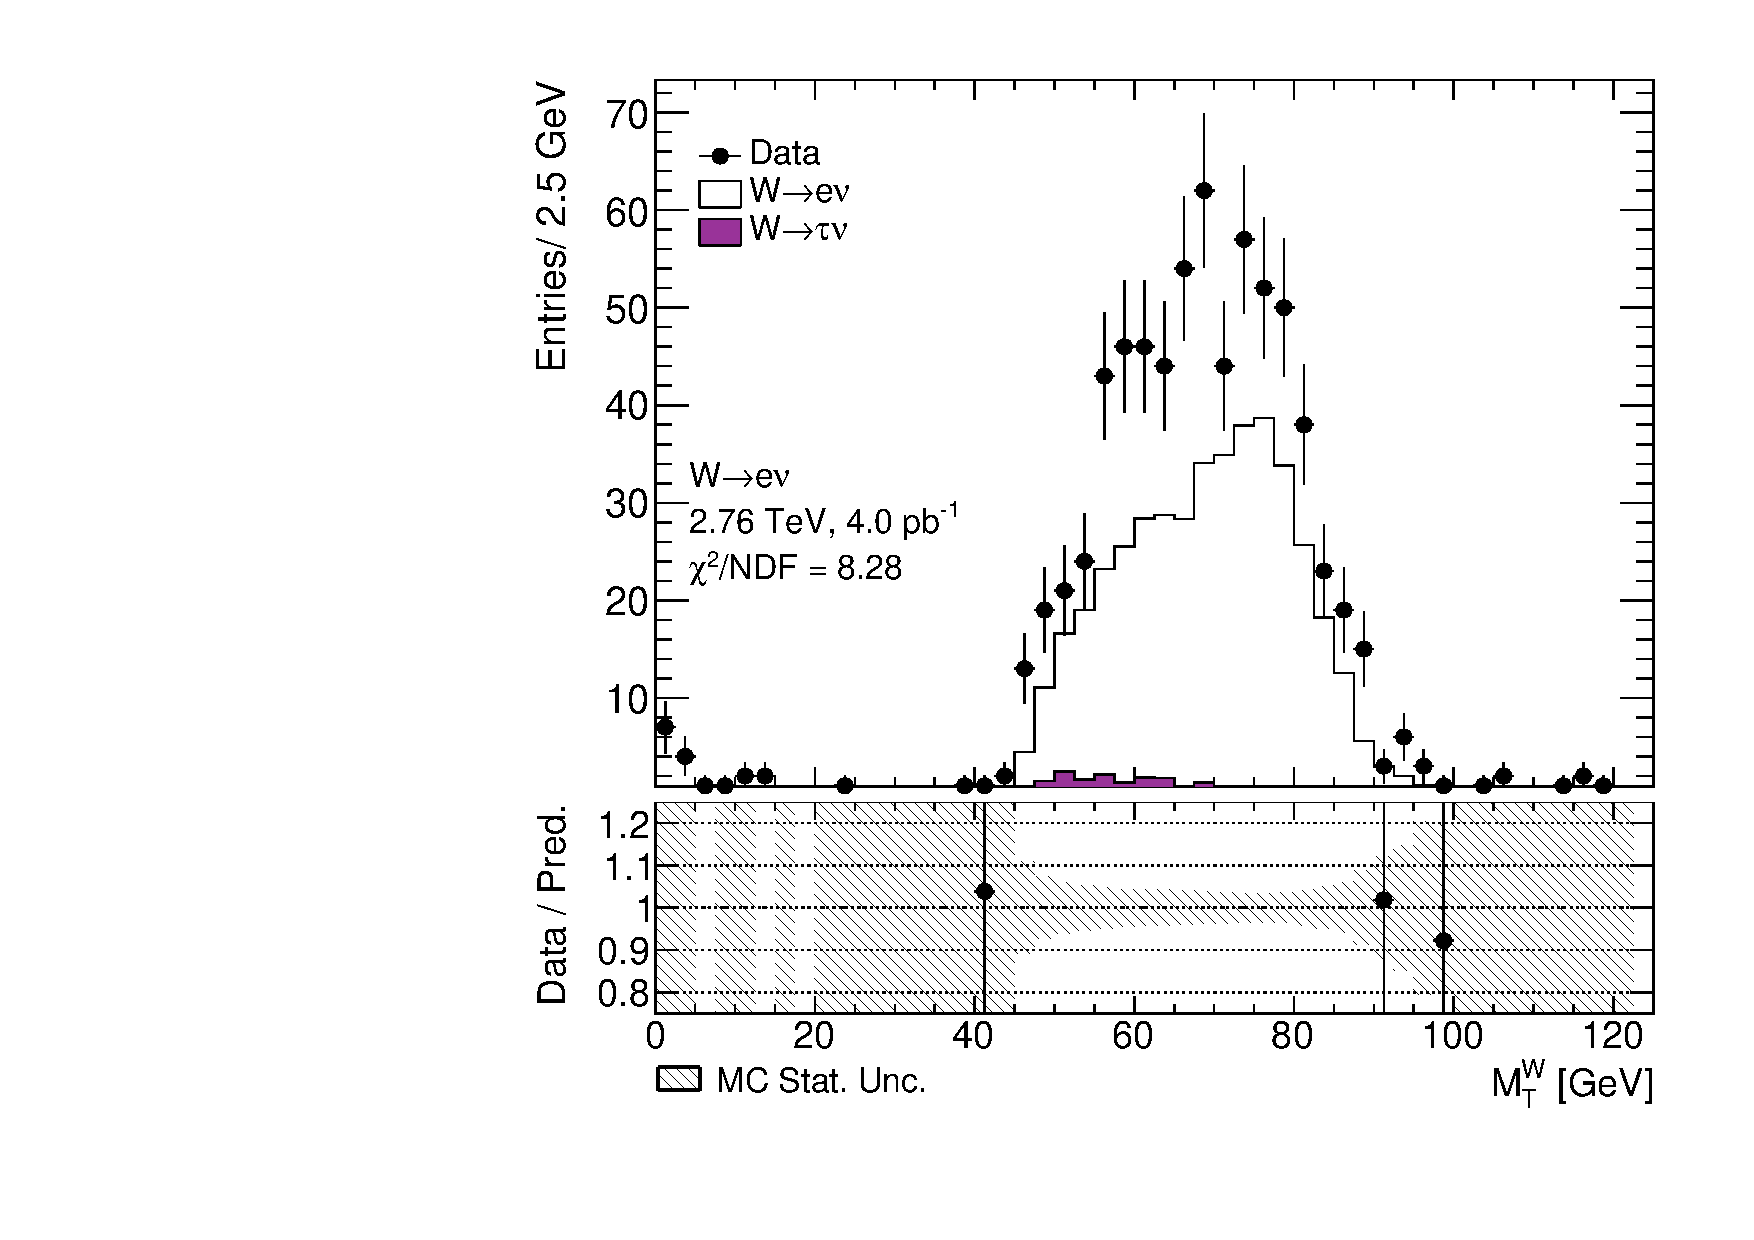
\includegraphics[width=1.\linewidth] {QCD/QCDmtWTempl.pdf} \\b)}
\end{minipage}
\caption{Distribution for a) missing transverse energy \etmiss b)mass transverse \mtw from the QCD template selection for \wenu events}
\label{ris:TemplateE}

\vfill

\begin{minipage}[h]{0.49\linewidth}
\center{ 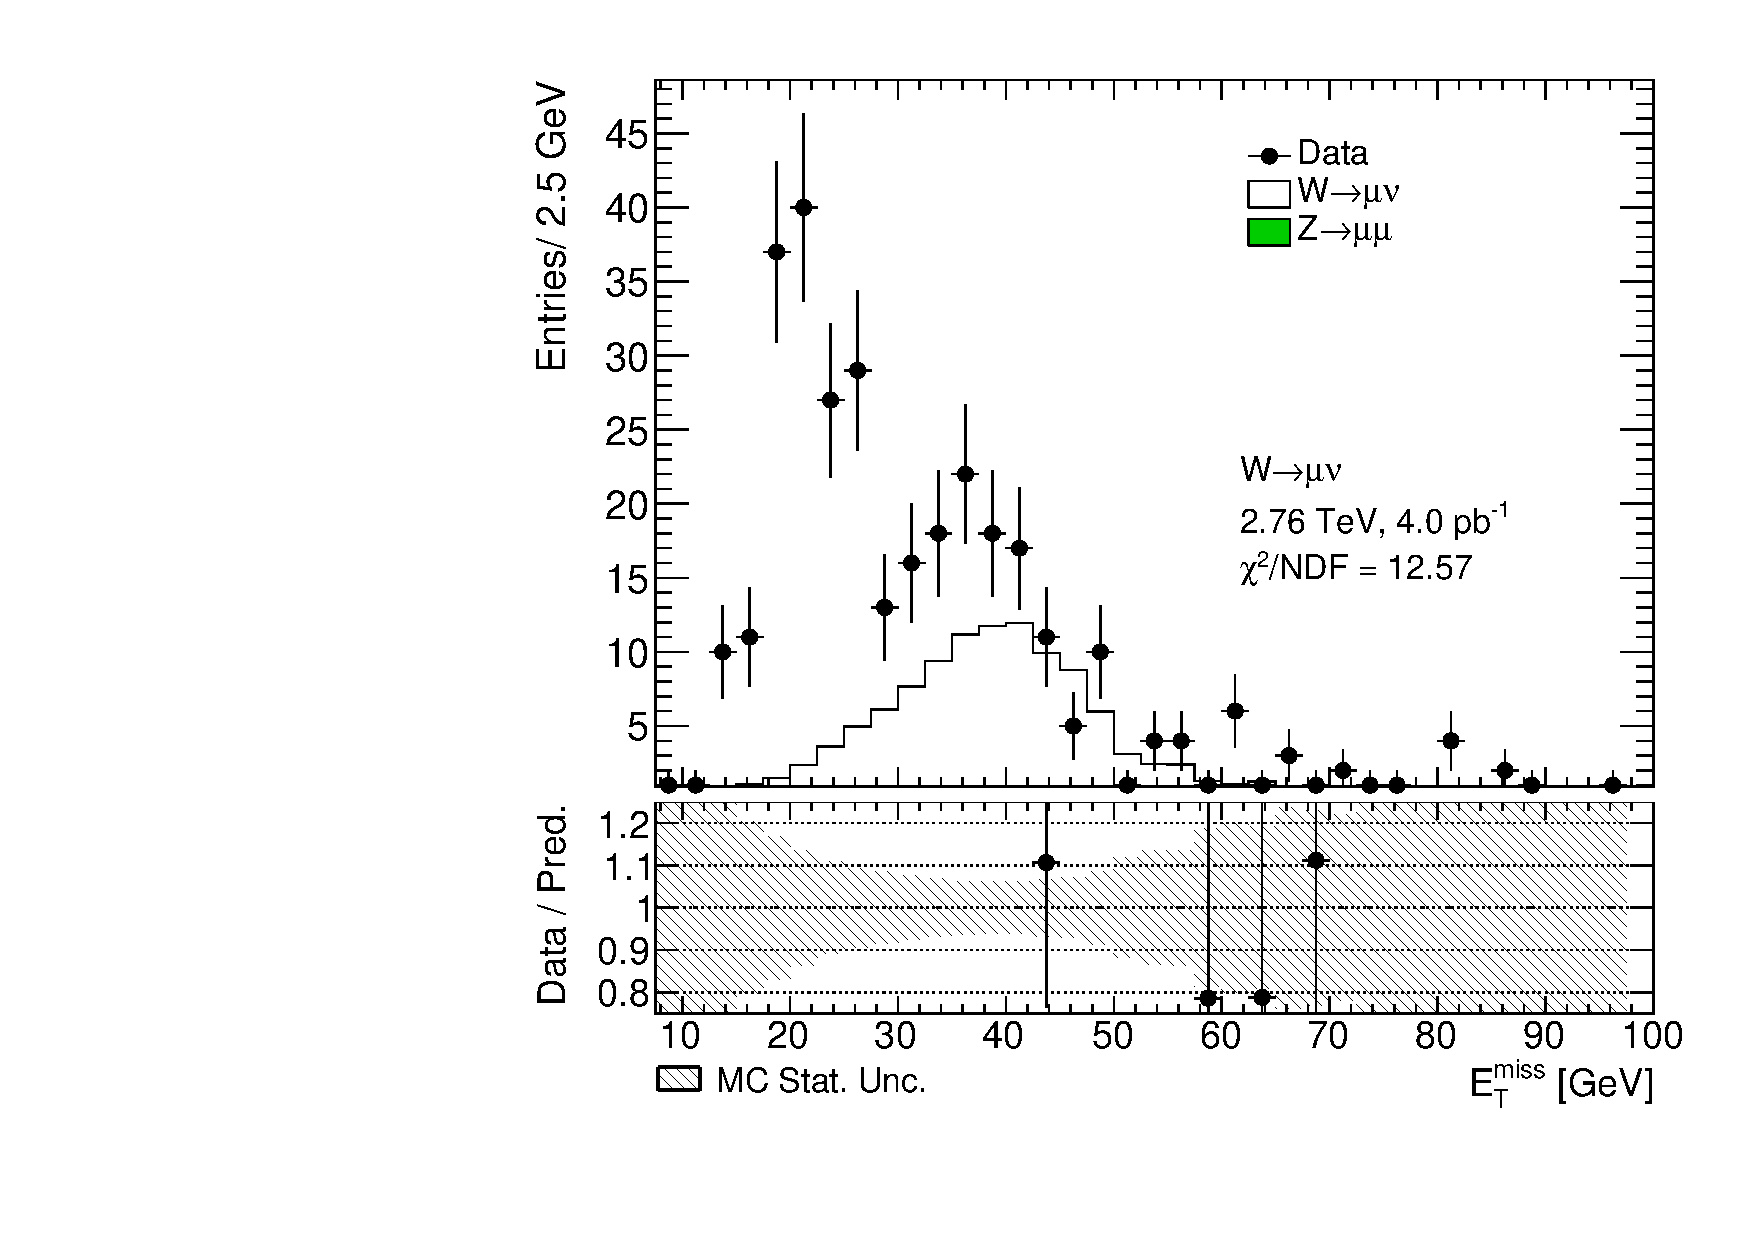
\includegraphics[width=1.\linewidth]{QCD/QCDWmuetMissTempl.pdf} \\a)}
\end{minipage}
\hfill
\begin{minipage}[h]{0.49\linewidth}
\center{ 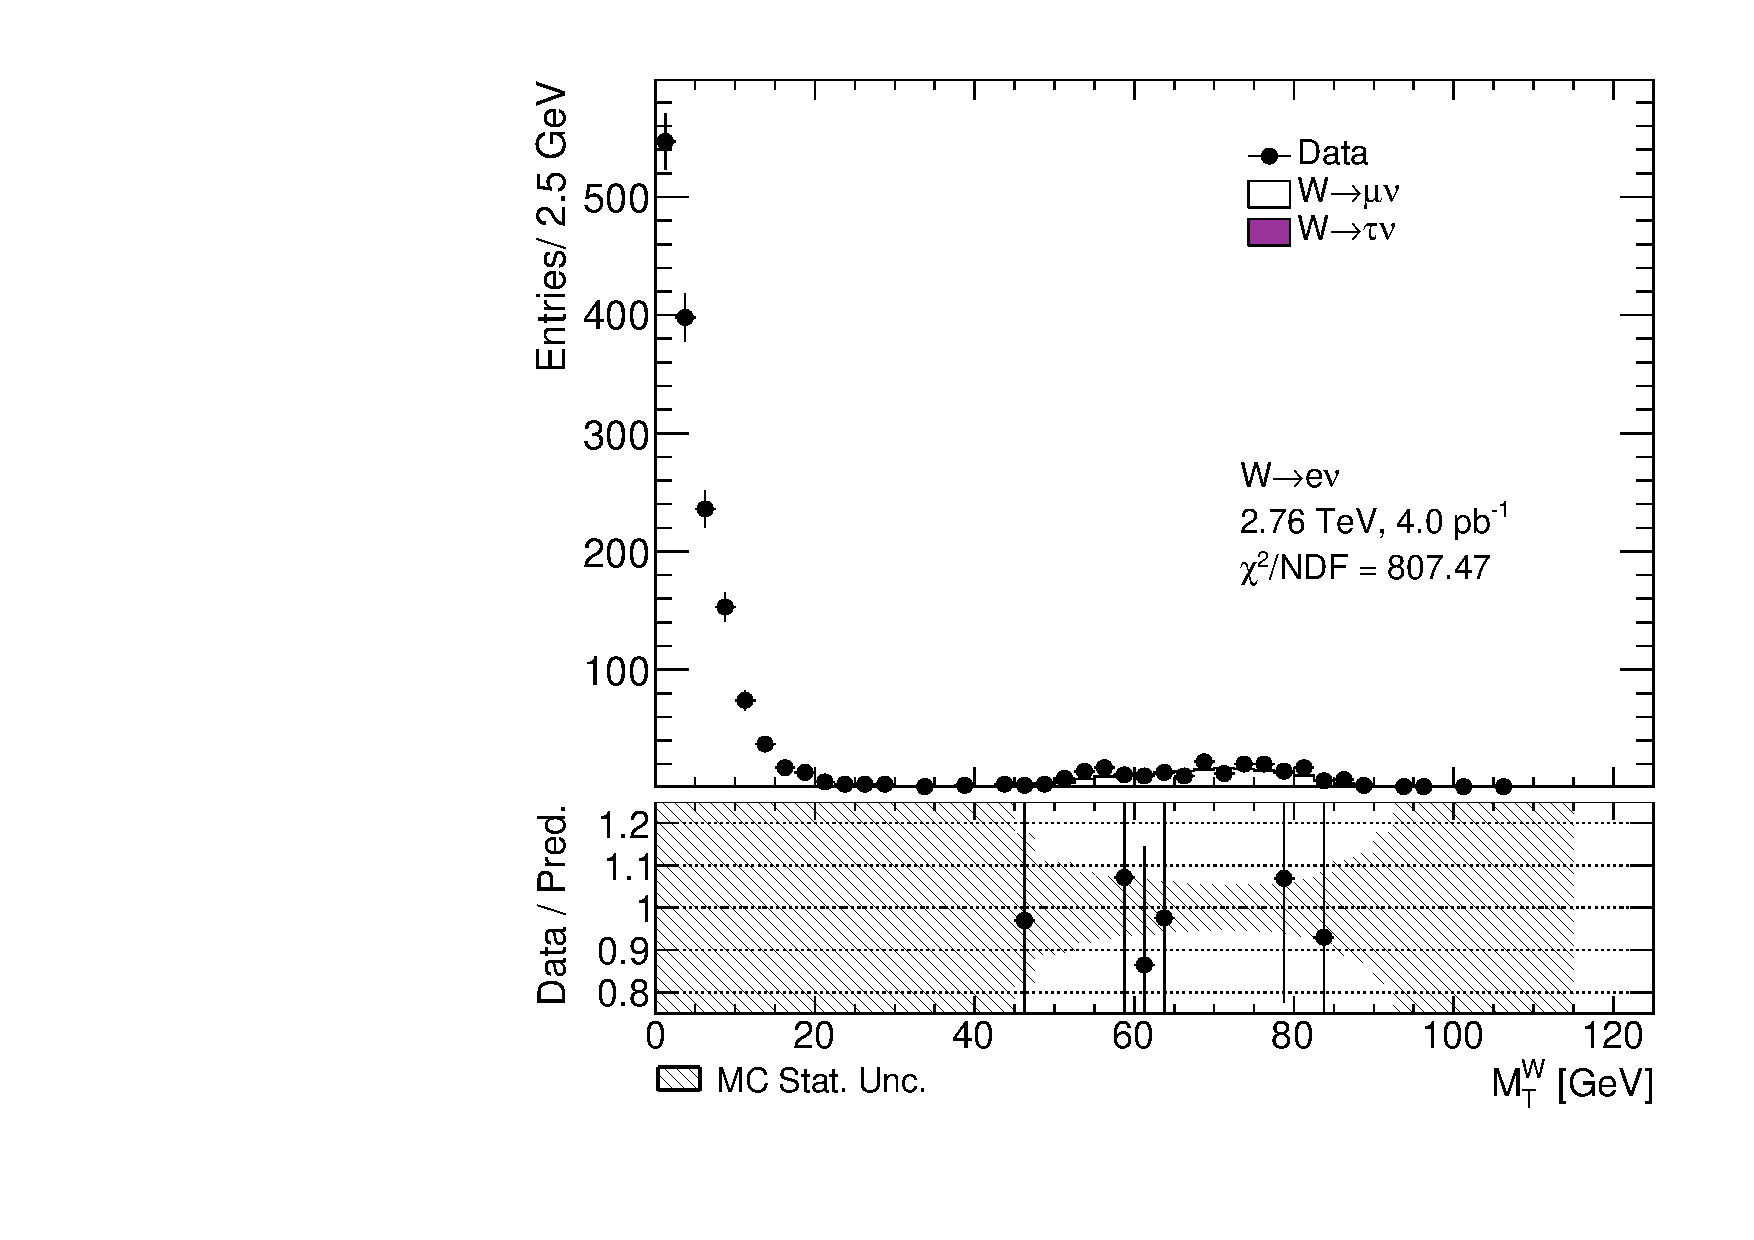
\includegraphics[width=1.\linewidth] {QCD/QCDWmumtWTempl.pdf} \\b)}
\end{minipage}
\caption{Distribution for a) missing transverse energy \etmiss b)mass transverse \mtw from the QCD template selection for \wmunu events}
\label{ris:TemplateMu}
\end{figure}

There is a small probability, that a jet can fake W-boson decay with isolated lepton and \etmiss through the energy mismeasurment in the event.  Event selection is suppressing this type of background, but not fully eliminating it. Due to a large jet production cross-section and complex composition, generation of MC events becomes impractical. This is why data driven technique for QCD background estimation have been used. In our case contribution from the QCD background  in the Z sample is negligible(Fig. \ref{fig:CPMassZ}), so it is estimated just for \wenu and \wmunu processes. 

Data driven method allows to have model independent predictions with small statistical uncertanty. This method is using \qcd enriched region, where signal events are supressed. This is usually done by reversing identification or isolation criteria. It is assumed, that shape of the \qcd background stays the same in the signal region. Normalization can  be derived in a control region through the template fit. 

This section describes method of \qcd background determination, that have been used in 2.76 TeV data. 

\subsection{Template selection}

A study have been performed to determine appropriate template selection. Because of the origin of the QCD backgrounds, missing transverse energy \etmiss should be smaller in background sample, that in a signal region. Releasing \etmiss cut allows to gain a bigger statistics for a QCD template. Another possibility is to relax the transverse mass \mtw cut. Most of the multijet background event should contribute to the small \mtw region. The template sample can contain also contributions from other backgrounds (mostly coming from \wlnu). The best template selection should allow for big data statistics and small electroweak contributions at the same time. In order to supress the signal additionally reversed ID or isolation criteria is applied. 

In electron channel, the template selection requires an electron candidate to fail medium identification criteria, but to pass loose selection. Control distributions for a different template selection in electron channel are shown on a Fig. \ref{ris:TemplateE}. Relaxed \etmiss cut allows to gain bigger template statistics. 

In a muon channel template selection is build by inverting isolation criteria ( \ptcone > 0.1). In case of \wmunu the \qcd background template the best statistics is achived by relaxing mass transverse \mtw cut (Fig. \ref{ris:TemplateMu}). 

In order to avoid double counting, electroweak processes (i.e. signal and backgrounds) are substracted from a template. The total number of events in the template can be defined as:
\begin{equation}
N_{template} = N^{bkg\, enriched}_{data} - \sum_{j}^{MC} N_{MC_j}^{bkg\, enriched},
\end{equation}
where $N^{bkg enriched}_{data}$ and $N_{MC_j}^{bkg enriched}$ are numbers of the events in a background enriched sample in data and different MC samples. The resulting template statistic is 1348 and 1509 events for \wenu and \wmunu respectively. 


\subsection{Methodology of the template sample normalization}

\begin{figure}[!tbp]
\begin{minipage}[h]{0.49\linewidth}
\center{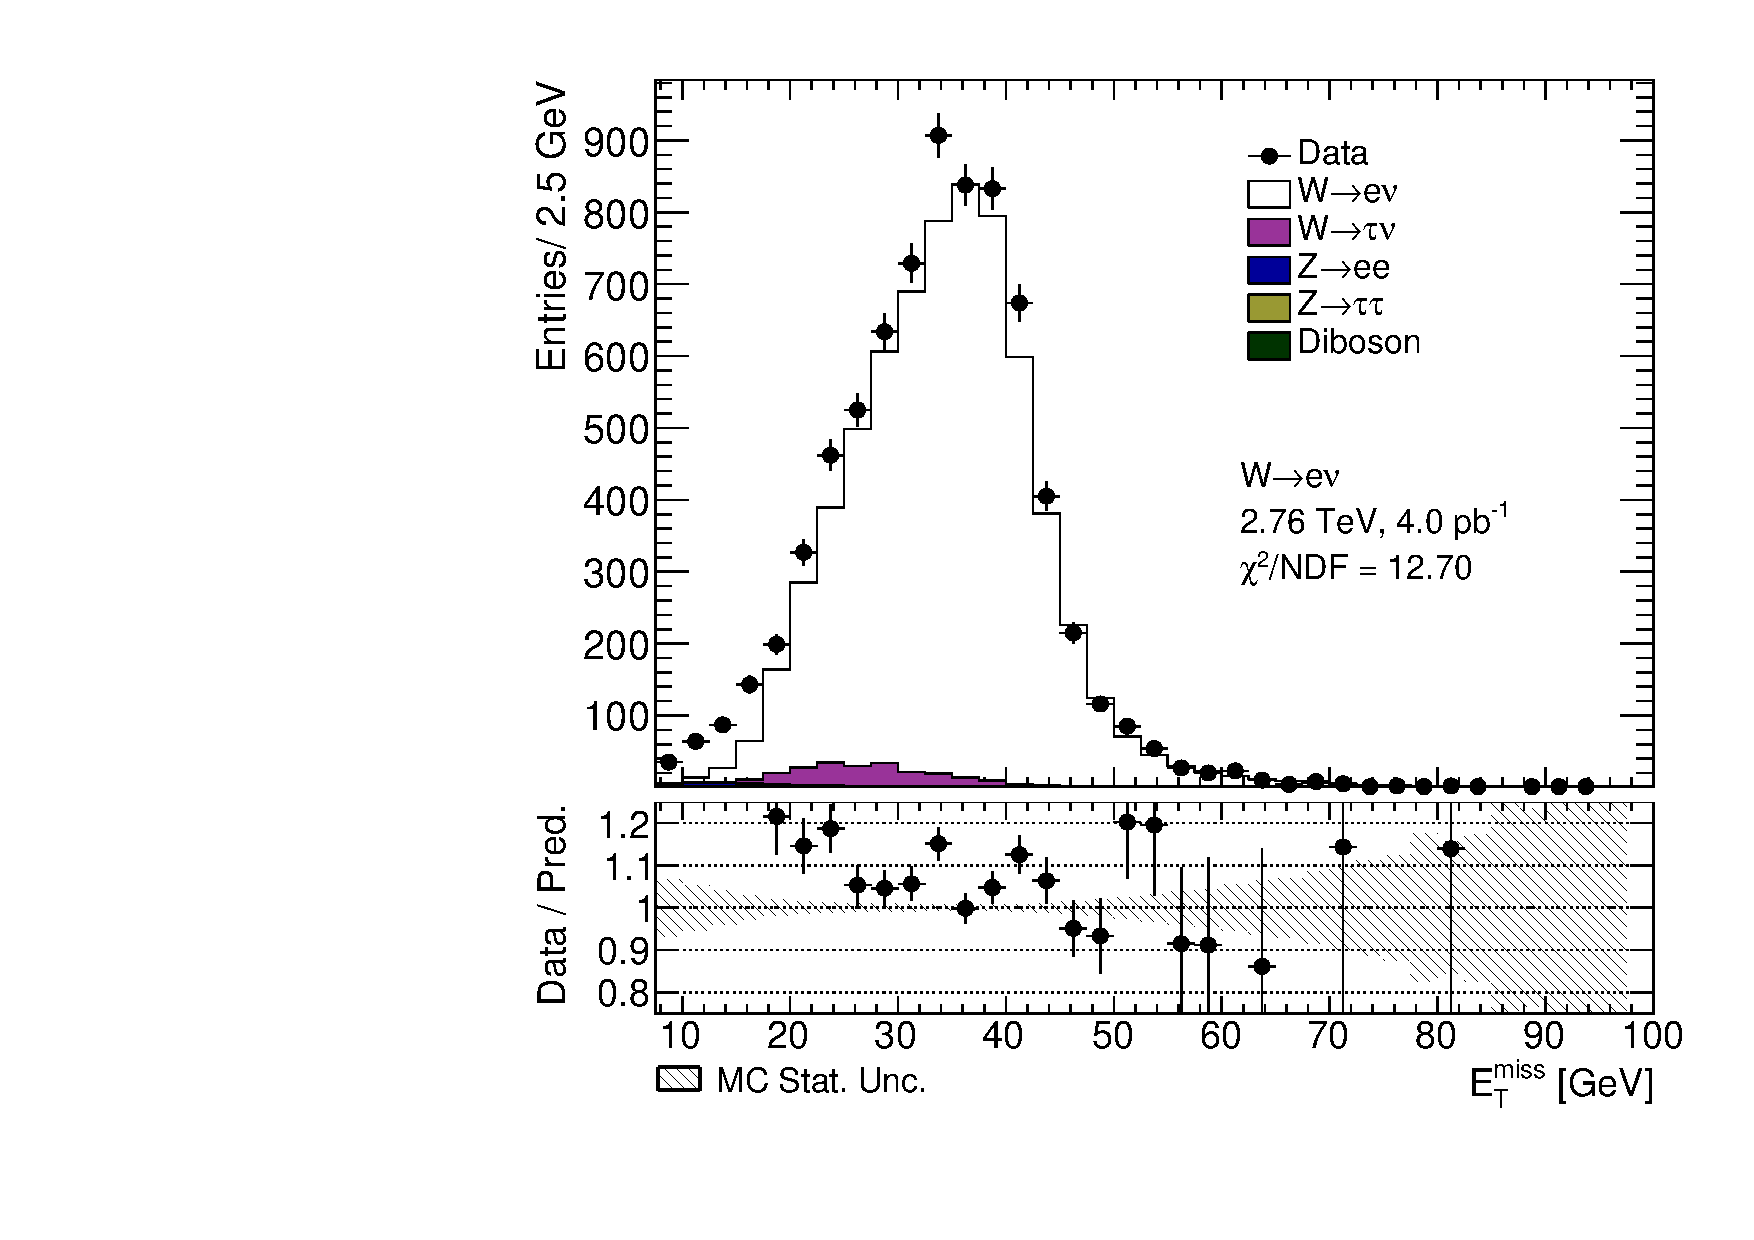
\includegraphics[width=1.\linewidth]{QCD/QCDetMissFit.pdf} \\ a)}
\end{minipage}
\hfill
\begin{minipage}[h]{0.49\linewidth}
\center{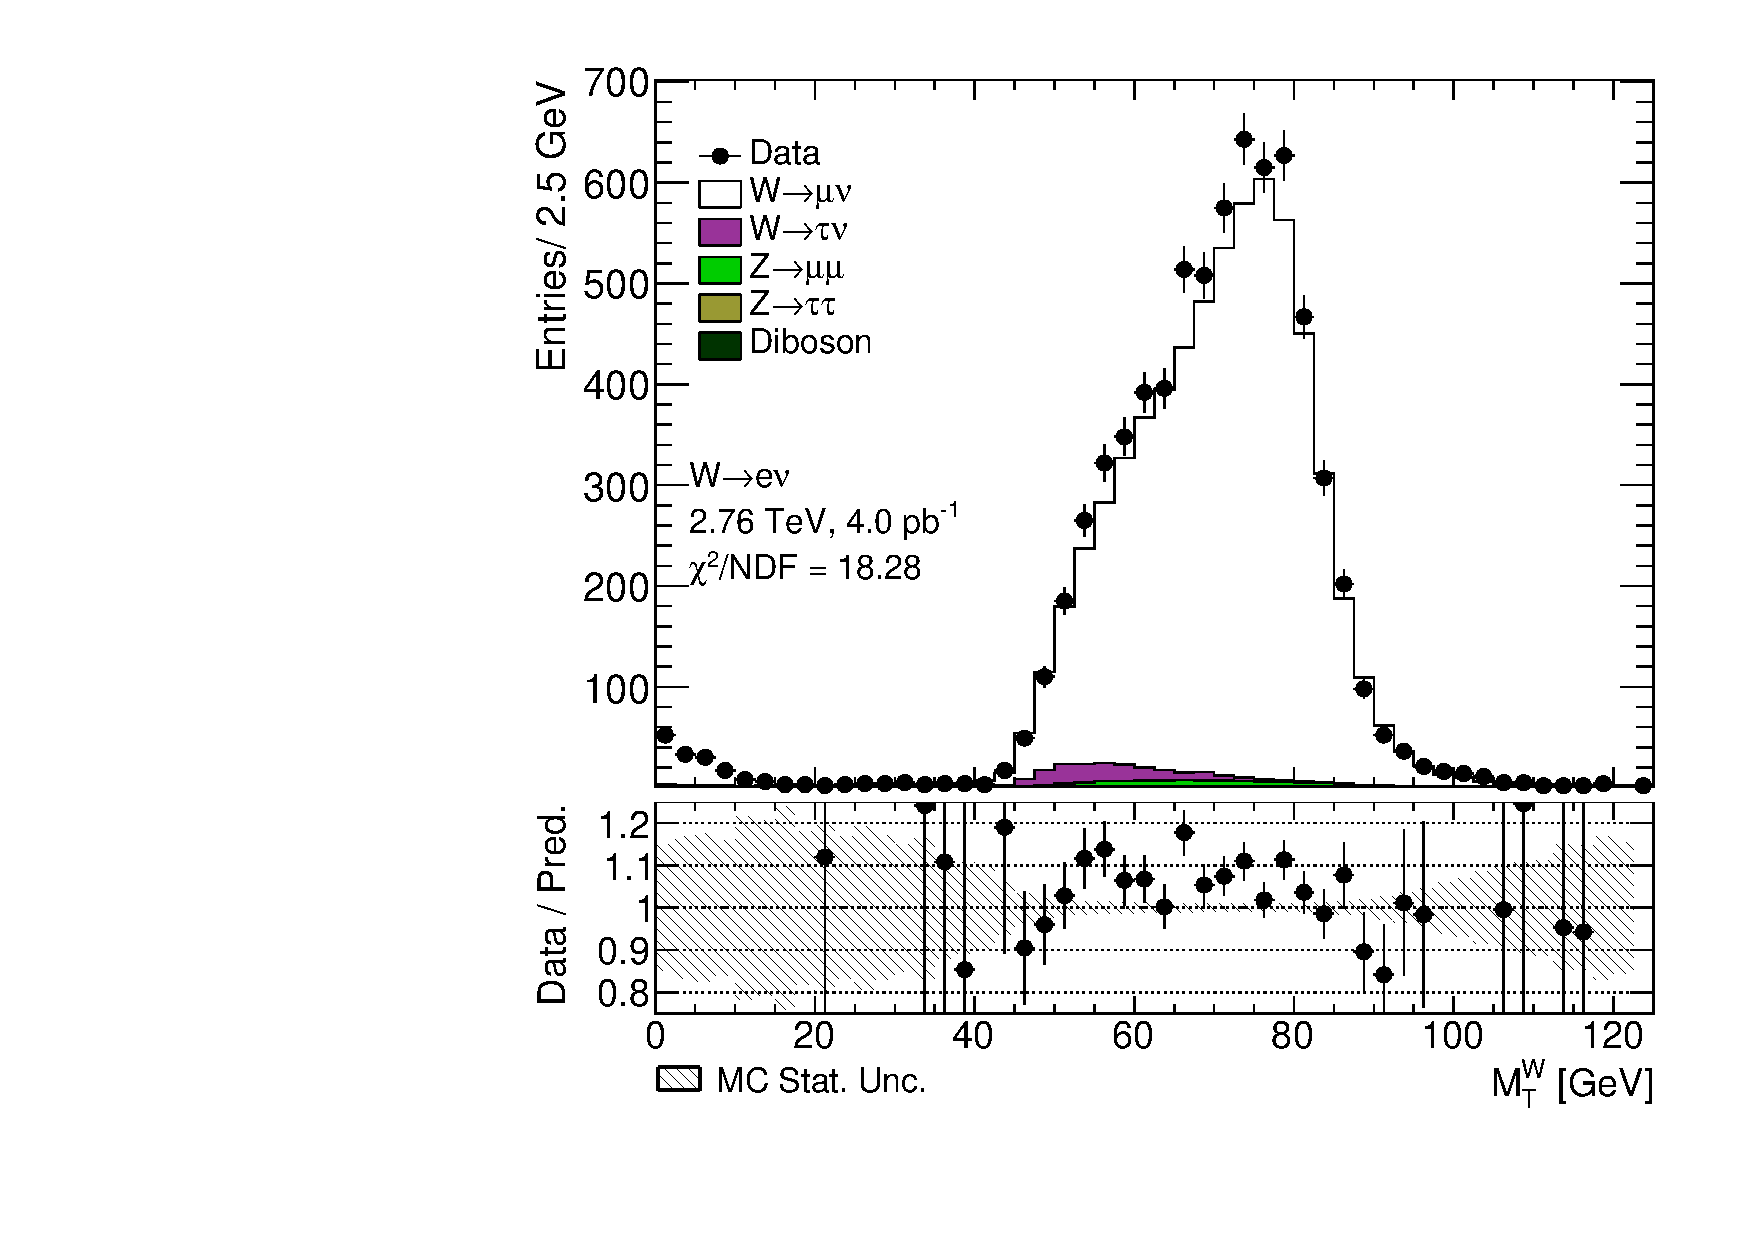
\includegraphics[width=1.\linewidth]{QCD/QCDWmumtWFit.pdf} \\ b)}
\end{minipage}
\caption{Distributions used for multijet background estimation for a) \wenu b)\wmunu}
\label{ris:FitDistributions}
\end{figure}

The normalization is found through the \chiD fit of the template and backgrounds to the data. The following composite model has been used for estimation:
\begin{equation}
M(x) = \sum_{i=1}^{N-1}f_iF_i(x) + (1- \sum_{i=1}^{N-1} f_i)\cdot F_{QCD}(x),
\end{equation}
where index i goes over the MC samples, $x$ is a fit variable (\etmiss or \mtw), $F_i(x)$ and $ F_{QCD}(x)$ are the probability density functions of MC samples and QCD background template respectivelly. Fit parameters $f_i$ are the fractions of MC events within the fit region. In order to eliminate systematics, coming from the cross-section uncertanty, the signal fractions are left as free parameters of fit and and the background MC fractions are allowed to be varied within 5\% uncertainty. 

Normalisation scale of the QCD events is calculated from the obtained fit parameters as:
\begin{equation}
scale = \frac{(1-\sum f_i) \cdot N^{fit}_{Data}}{N_{template}},
\end{equation}
where $\sum f_i$ is a sum of all fractions in the fit, $N^{fit}_{Data}$ is a number of data events in a fit histogram and $N_{template}$ is a number of event in a template. The fit is performed separatelly for $W^{+}$ and $W^{-}$. Additionally, fit in total $W$ channel is used as a cross-check of the fit.
The results of the fitting procedure are shown on a Fig. \ref{ris:Fit} . 
 
\begin{figure}[!tbp]
\begin{minipage}[h]{0.49\linewidth}
\center{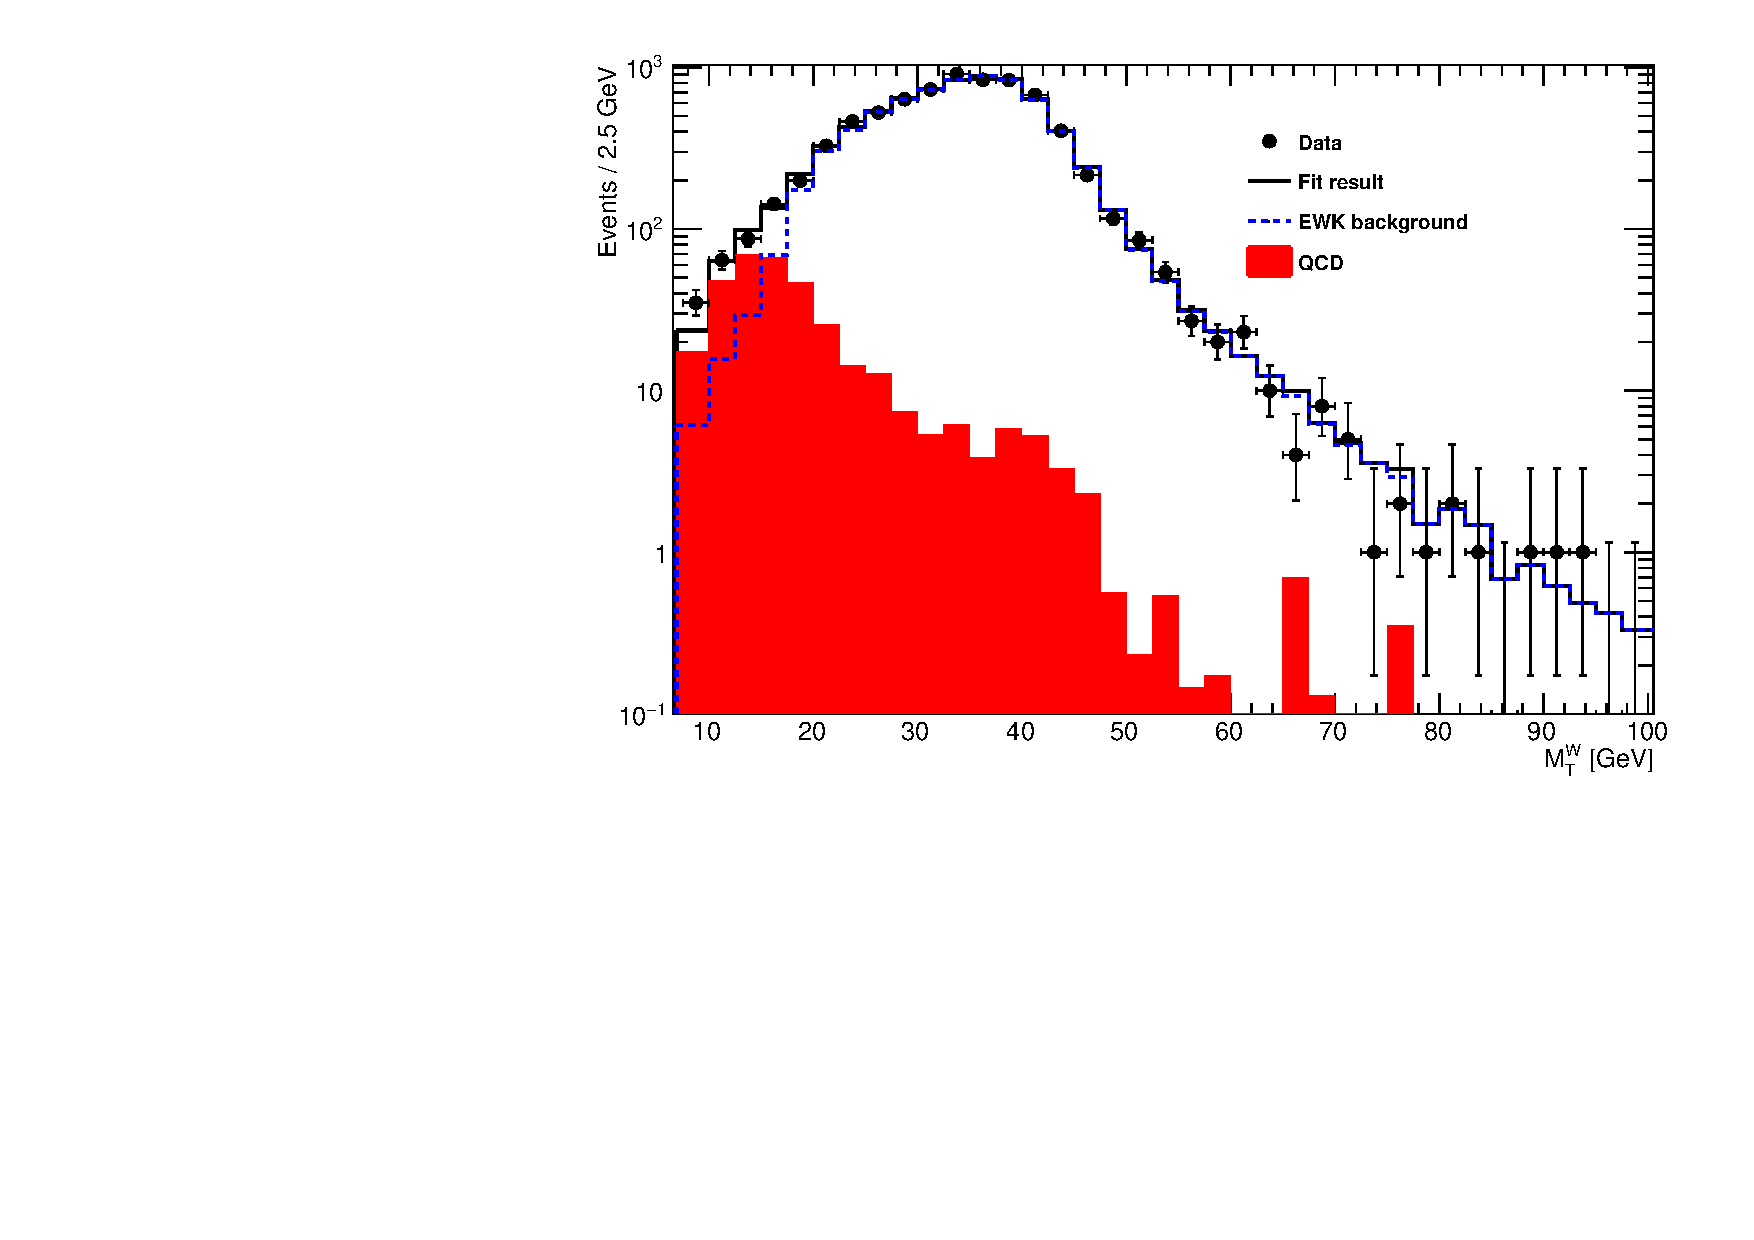
\includegraphics[width=1.\linewidth]{QCD/etMissFit.pdf} \\ a)}
\end{minipage}
\hfill
\begin{minipage}[h]{0.49\linewidth}
\center{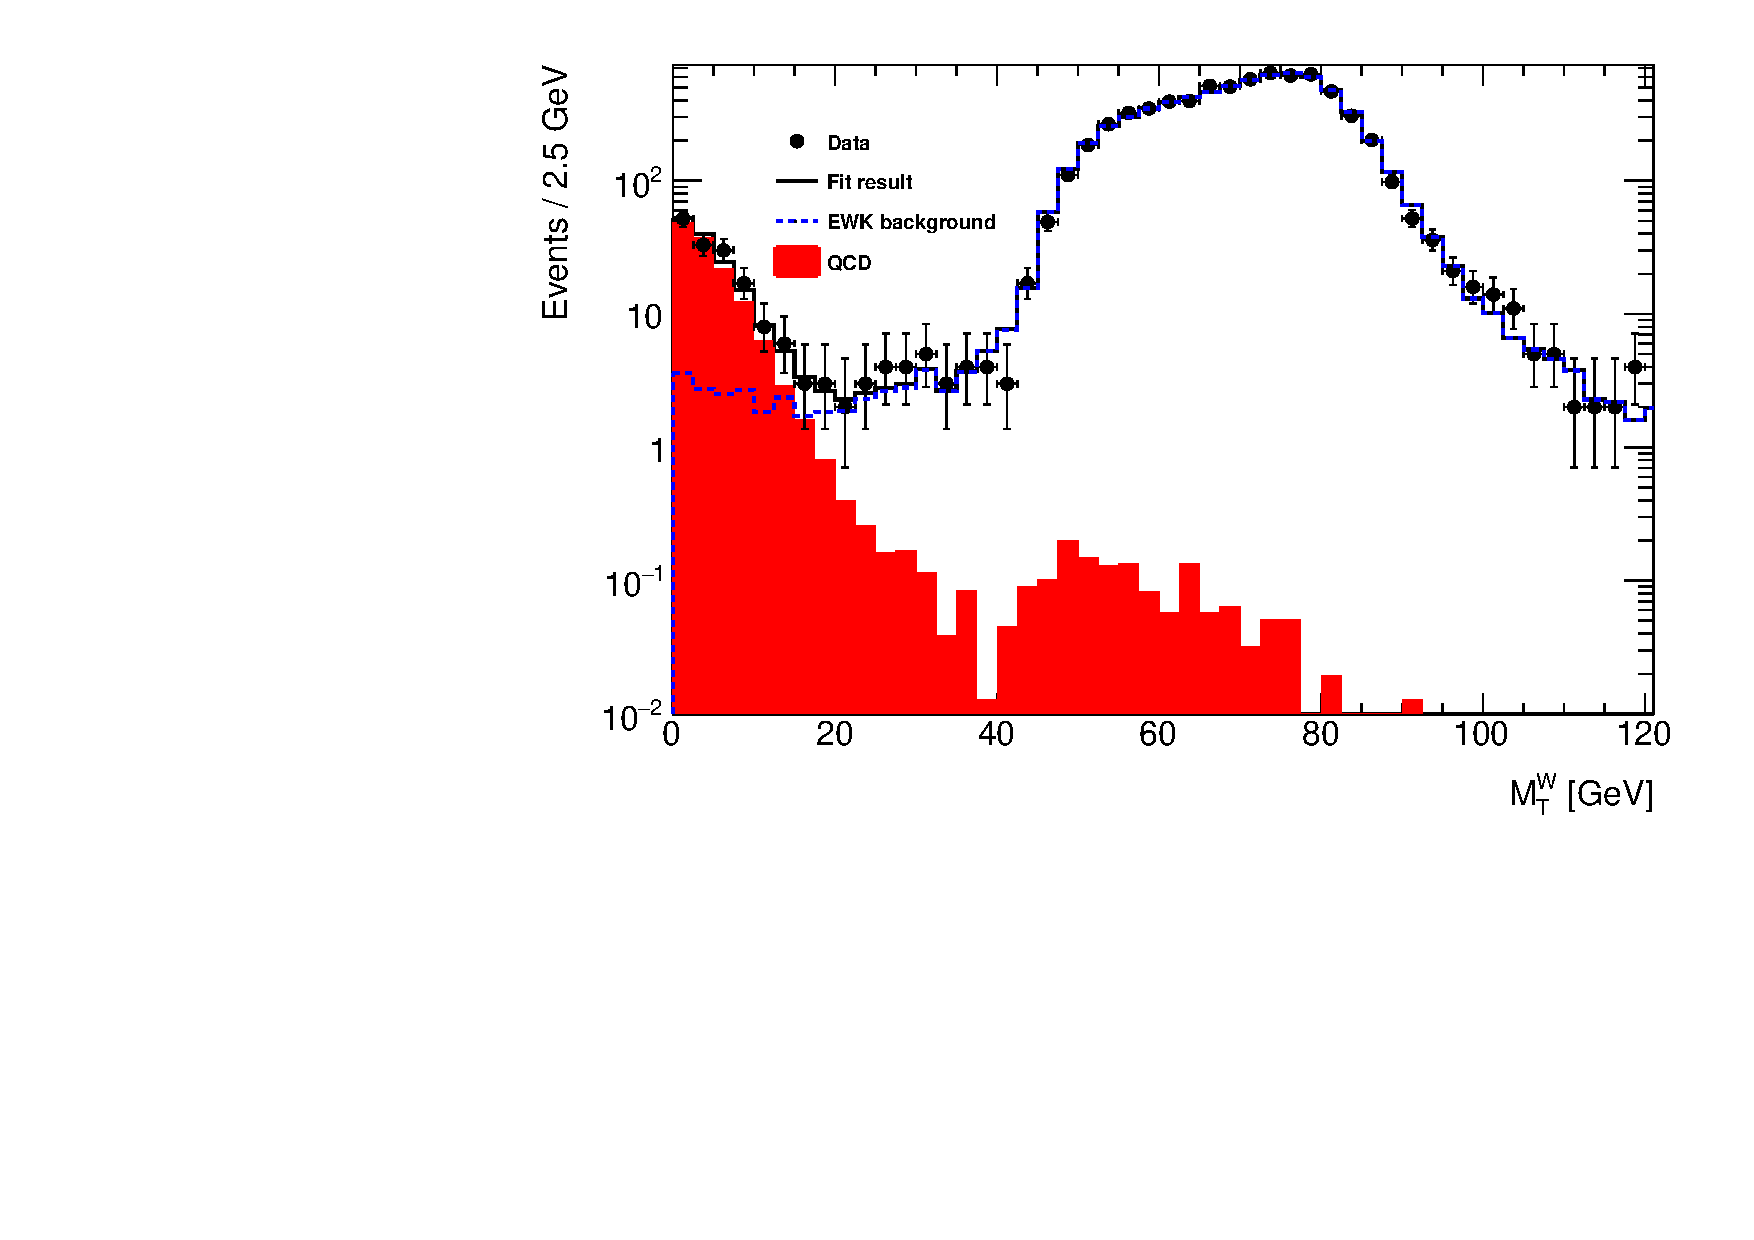
\includegraphics[width=1.\linewidth]{QCD/MtWFit.pdf} \\ b)}
\end{minipage}
\caption{The multijet background estimation for a) \wenu using reversed ID cut and released \etmiss cut b) \wmunu using released \mtw cut and $b\bar{b}+c\bar{c}$ template}
\label{ris:Fit}
\end{figure}

\subsection{Systematic uncertainty from the multi-jet background estimation }\label{sec:QCDUnc}

The uncertanty of the multi-jet background estimation can be divided into 3 main components:
\begin{equation}
\delta_{QCD} = \sqrt{ \delta_{fit\, unc}^{2}+\delta_{MC}^{2}+\delta_{fit\, bias}^{2}+\delta_{template}^{2}}, 
\end{equation}
where $\delta_{fit\, unc}$ is the uncertanty for a scale from a \chiD fit. The meaning of other components is explained below

The second component $\delta_{MC}$ is coming from a possible mismodelling of MC in a fitted region. It can be estimated by comparison of fit results for $W$, $W^{+}$ and $W^{-}$. Number of multijet background events should not depend on a charge of the analysis, so it is expected:
\begin{equation}
N_{QCD}^{W}=0.5 \cdot N_{QCD}^{W^{+}} =N_{QCD}^{W^{-}}
\end{equation}
Standard deviation of these 3 numbers is taken as systematic uncertainty. Since in \wmunu channel the QCD template normalization is derived from the fit in small \mtw region, where electroweak contributions negligible and data statistics is high, this systematic source is equal to 0.

\begin{figure}[!tbp]
\begin{minipage}[h]{0.49\linewidth}
\center{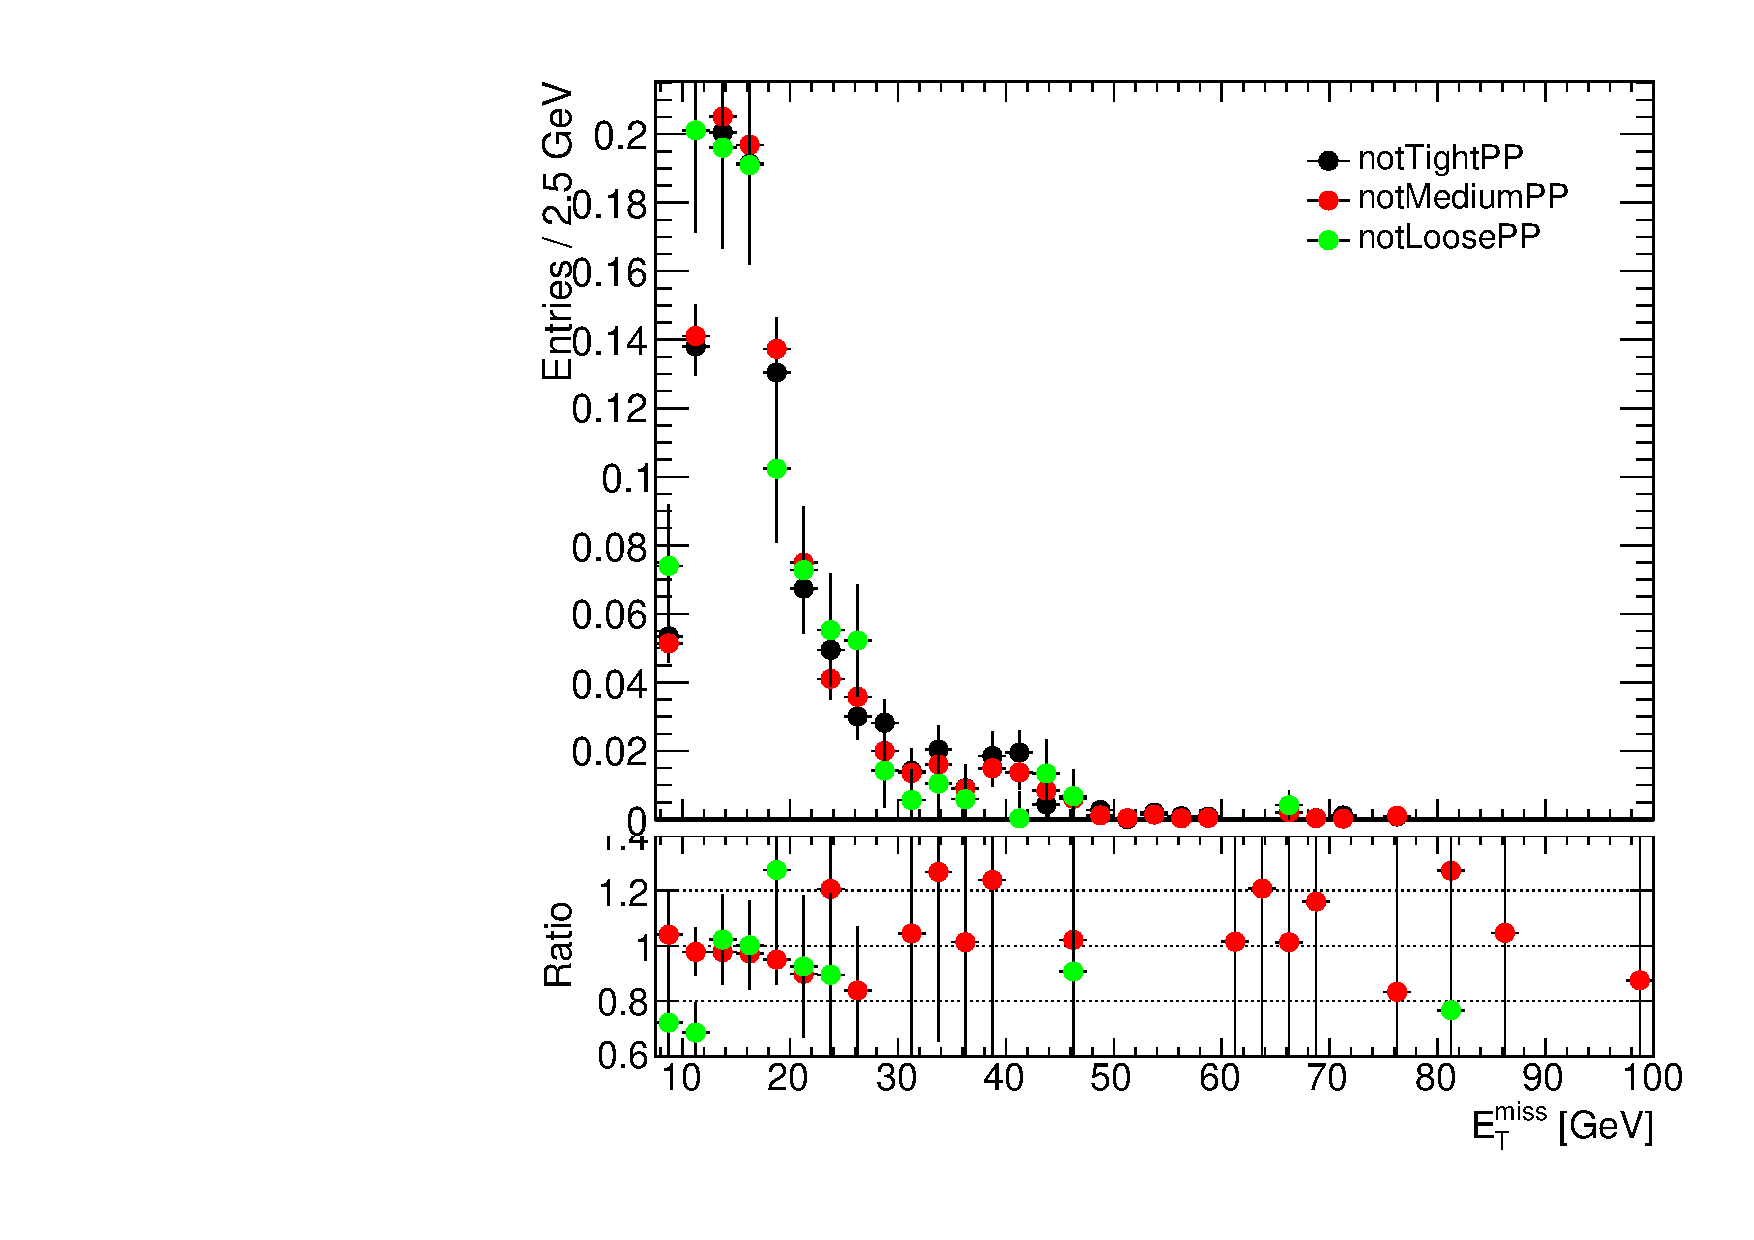
\includegraphics[width=1.\linewidth]{QCD/ElecTemplates.pdf} \\ a)}
\end{minipage}
\hfill
\begin{minipage}[h]{0.49\linewidth}
\center{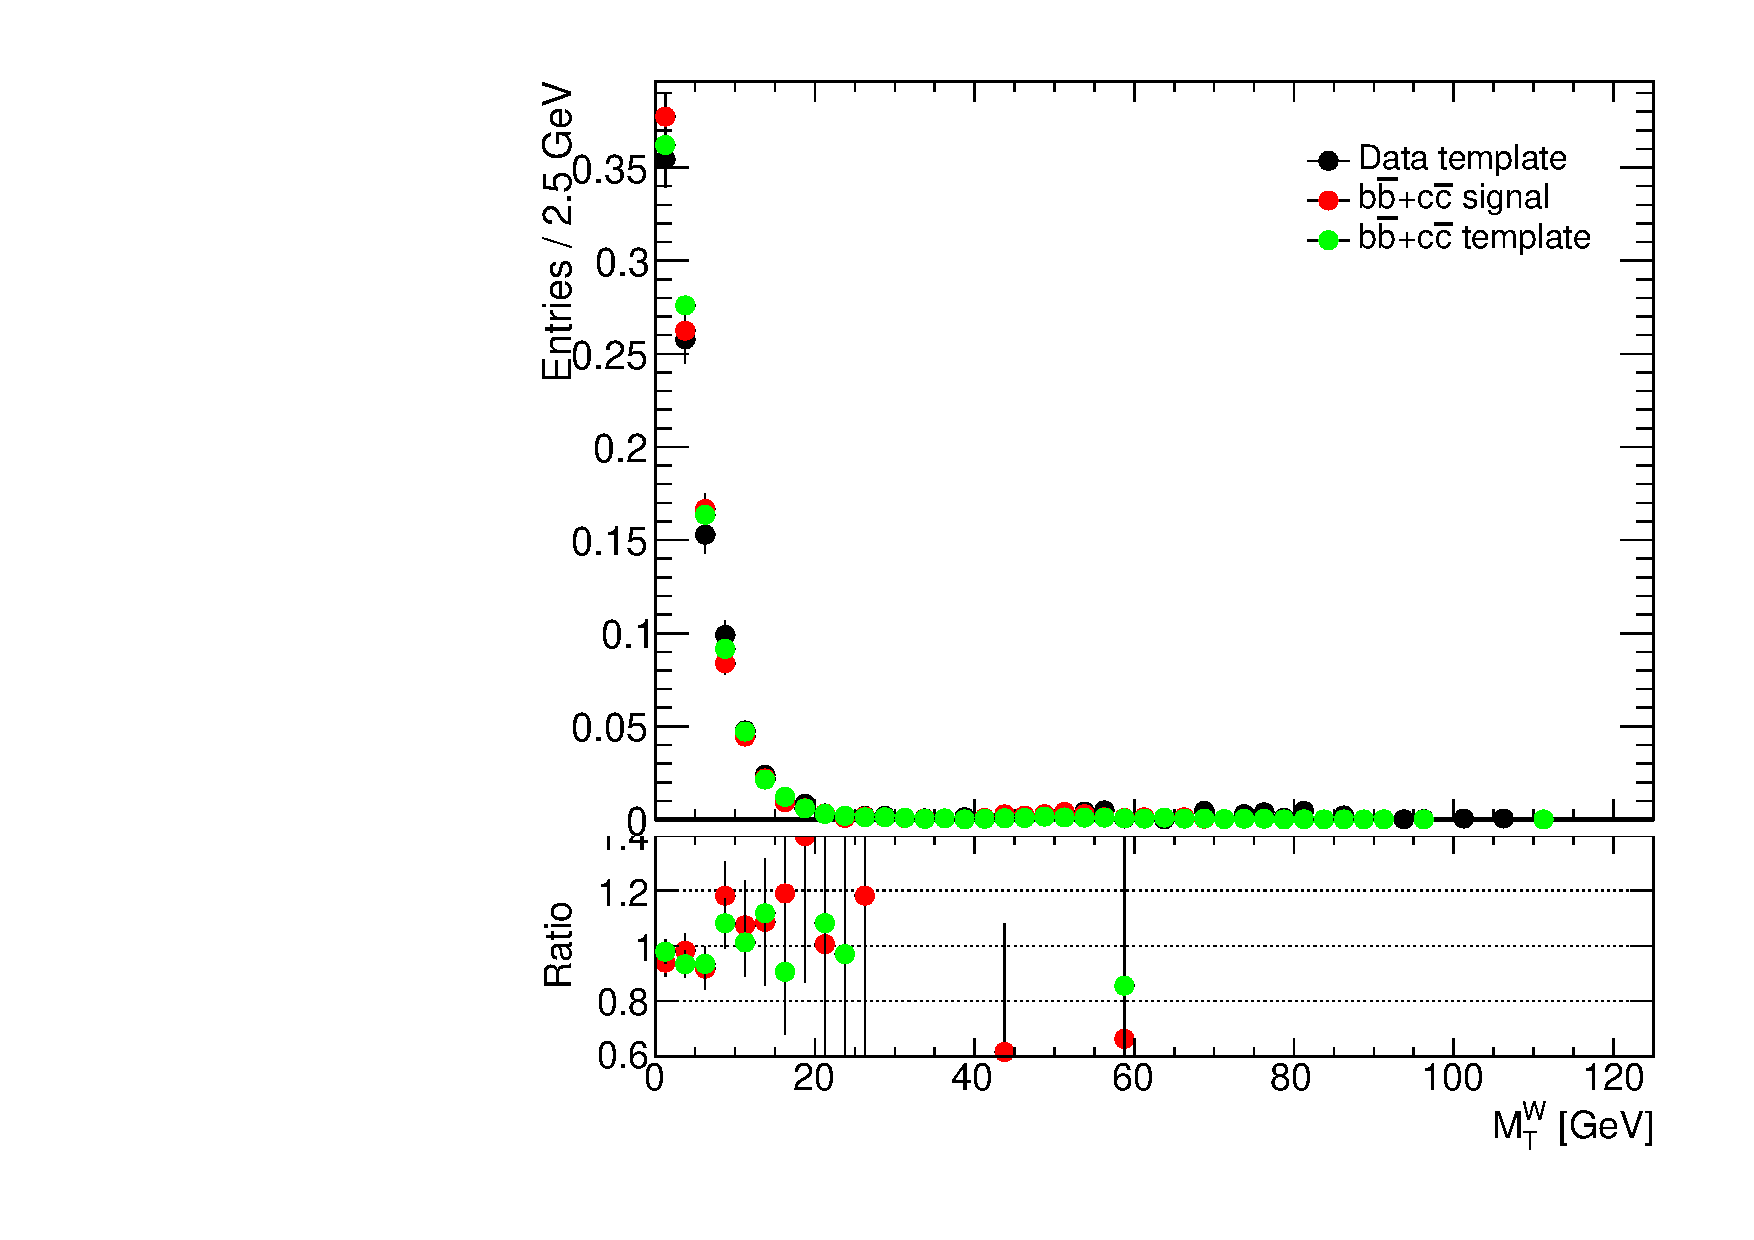
\includegraphics[width=1.\linewidth]{QCD/QCDBkgWmuTemplates.pdf} \\ b)}
\end{minipage}
\caption{Data and MC comparison for \etmiss calculated by standard \atlas algorithm for a)\wenu b)\wmunu events}
\label{ris:TemplateVar}
\end{figure}

The third component $\delta_{fit\, bias}$ is coming from an effect of an arbitrary choice of bin size . This error is estimated by repeating the fit for a different binnings. This component is assumed negligible in \wmunu case. 

The uncertainty $\delta_{template}$ is due to a potential bias in the template as a result of the template choise and a template statistics itself. For estimation of this uncertainty different template selections have been used. For \wenu channel different reversed isolation criteria have been tried (Fig. \ref{ris:TemplateVar} a)). The overall discrepancies can be considered negligible. For \wmunu channel template variations are estimated using fits with $b\bar{b}+c\bar{c}$ MC samples.  Fig. \ref{ris:TemplateVar} b) compares data template with template obtained using signal selection with released \mtw cut and template selection. Results for a different template fits are presented in Tab \ref{tab:QCDWmunu}



Results of the QCD background uncertainty estimation for \wenu and \wmunu are shown in Tab. \ref{tab:QCDWenu} and \ref{tab:QCDWmunu} respectively. The overall number of QCD background events is estimated as \nQCDWplusenu\,  for $W^{+}\to e^{+}\nu$ and $W^{-}\to e^{-}\nu$ and \nQCDWplusmunu\,   for $W^{+}\to \mu^{+}\nu$ and $W^{-}\to \mu^{-}\nu$. The overall fraction of the QCD events is lower, than in 13 TeV \cite{a13TeV}, 8 TeV \cite{a8TeV} and 7 TeV \cite{a7TeV} data, what is in agreement with expectations.

\begin{table}[!tbp]
    \caption{Results of QCD background estimation for \wenu and corresponding error}
	\label{tab:QCDWenu}
	\begin{center}
		\begin{tabular}{l | c | c | c | c }
		\hline
		    Charge & $N_{QCD}$ & $ \delta N_{fit\, unc} $ & $\delta N_{MC}$ & $\delta N_{fit\, bias}$ \\
		    \hline
		    $W^{+}$ & 38.3 & 7.0 & 7.0 & 5.0 \\
		    $W^{-} $ & 21.5 & 0.7 &  -9.4 & 4.0 \\
		    $W$ & 66.1 & 21.2 & 4.2 & 10.  \\
		    \hline
		    \hline
		    Total & 31.0 & 6.1 & 8.6 & 4.7 \\
		    \hline
		\end{tabular}
	\end{center}
\end{table}

\begin{table}[!tbp]
    \caption{Results of QCD background estimation for \wmunu using different templates and it's fit error}
	\label{tab:QCDWmunu}
	\begin{center}
		\begin{tabular}{l | c | c | c  }
		\hline
		    Charge & $N_{QCD}$ & $N_{QCD}$ & $N_{QCD}$ \\
		    & data template & $b\bar{b}+c\bar{c}$ template selection & $b\bar{b}+c\bar{c}$ signal selection \\
		    \hline
		    $W^{+}$ & 2.48 & 0.73 & 1.34 \\
		    $W^{-} $ & 2.48 & 0.73 & 1.35 \\
		    $W$ & 4.97 & 1.47 & 2.70  \\
		    \hline
		    \hline
		    Total per channel & 2.48 & 0.73 & 1.35 \\
		    Fit error & 0.60 & 0.73 & 0.19 \\
		    \hline
		\end{tabular}
	\end{center}
\end{table}

\begin{table}[!b]
    \caption{Number of observed candidate events for the $W \to l\nu$ channel, electroweak (EWK) and top, and data-driven QCD background events, and background-subtracted signal events}
	\label{tab:BkgWlnu}
	\begin{center}
		\begin{tabular}{l || c || c | c || c  }
		\hline
		l & Observed & Background & Background & Background-subtracted \\
		 & candidates & (EWK + top) & (Multijet) & data $N_{W}^{sig}$ \\
		 \hline
		 \hline
		 & \multicolumn{4}{c}{W boson}\\
		 \hline
		 $e^{+}$ & \ntotWplusenu & \nEWttbarbkgWplusenu & \nQCDWplusenu & \ntotsignalWplusenu \\
		 $e^{-}$ & \ntotWminenu & \nEWttbarbkgWminenu & \nQCDWminenu & \ntotsignalWminenu \\
		 $\mu^{+}$ & \ntotWplusmunu & \nEWttbarbkgWplusmunu & \nQCDWplusmunu & \ntotsignalWplusmunu \\
		 $\mu^{-}$ & \ntotWminmunu &\nEWttbarbkgWminmunu & \nQCDWminmunu & \ntotsignalWminmunu \\
		 \hline
		 \hline
		 & \multicolumn{4}{c}{Z boson}\\
		 \hline
		 $e$ & \ntotZee & \nEWttbarbkgZee  & - &\ntotsignalZee \\
		 $\mu$ & \ntotZmumu &\nEWttbarbkgZmumu  & - & \ntotsignalZmumu \\
		 \hline
		 \end{tabular}
   \end{center}
\end{table}

\section{Background-subtracted W and Z candidate events}

Tables \ref{tab:BkgWlnu} summarize the number of background events for W and Z selections. Uncertanties on a number of EWK+top events are coming from a statistics, cross-section uncertainty (if given) and 3\% of luminosity determination uncertainty. For multijet background uncertainty is coming from a method and described in a subsection \ref{sec:QCDUnc}. For the background-subtracted events the statistical uncertainty is quoted first, followed by the total systematic uncertainty, derived from the EWK+top and multijet bacgrkound ones, considering the sources as uncorrelated. 



